\chapter{Datastream Extraction Tool Manual} \label{appendix-dset-manual}
\captionsetup{margin=10pt,font=large,labelfont=bf,textfont={bf}}

The full version of the Datastream Extraction Tool Manual can be found in the project folder of the Google Drive repository under \url{https://bit.ly/3rB3lqg}. 

\section{Introduction}
The Datastream Extraction Tool is an application that allows the user to download financial data from Thomson Reuters Datastream without the overhead of doing it manually in Excel. The tool was created specifically for large static and time-series requests, and supports long-duration downloads of data. 

\section{Installation}
Please, be aware of the following: 
\begin{itemize}
	\item The application can only be run on Windows computers. It cannot be ported to MacOS or Linux, as the Thomson Reuters Excel add-in is only available for Windows, and also because the VBA (Visual Basic for Applications) version on Unix-based computers is a different one than on Windows computers. 
	\item While the application can generally be run on remote computers as well, it can be rather inconvenient. On the one hand, remote computers tend to be less stable in terms of internet connection and add-in connectivity. And additionally, the remote computers of TUM-SOM have rather poor performance (especially disk access!), which would constrain the data download. Furthermore, remote computers automatically shut down after some time, which makes downloading large data loads problematic. For smaller requests though, that take up to 1 hour of download time, the remote execution should suffice. 
\end{itemize}

\subsection{Prerequisites}
Please make sure that the following environment is established before you proceed with the installation.
\begin{itemize}
	\item Make sure you have a valid \textbf{Microsoft Office Installation}. The application was tested with Office 365, but it should also run with other recent Office environments.
	\item Make sure that \textbf{Thomson Reuters Eikon \& Datastream} is installed. If you install it for the first time, please ensure that the Datastream add-on in the Excel plug-in is enabled. 
	\item Make sure that you have an up-to-date version of \textbf{Python 3} installed. Python 3 is different from Python 2; with Python 2 the application will not work. 
	\item Make sure that in Windows Power Options you select that your PC "never" goes to sleep. Since otherwise this can interrupt long-running downloads. 
\end{itemize}

\subsection{Download}
Follow these steps to install the application on your computer: 
\begin{enumerate}
	\item Download the \textit{Shippable} folder from \url{https://bit.ly/2VfT058} to your computer. Choose a location with enough free space, as the downloaded data will be stored in-place. 
	\item Unzip the downloaded file. You can rename the root folder from \textit{Shippable} to a different name at your convenience. Please, do \textbf{not} rename any of the folders or files inside. Such changes would need to be propagated to the program code. 
	\item In the \textit{Shippable }folder, you will find a file called \textbf{\textit{prerequisites.py}}. You need to run this file with Python. You can do so by e.g. right-clicking on the file, selecting "Open with" and then choosing Python. It will then automatically install external Python packages needed for the app. 
\end{enumerate}

\subsection{Settings}
Finally, you will need to adjust some settings in Excel the first time you install the application. For this purpose, open the file called \textit{RequestTable.xlsm} in the \textit{Shippabl}e folder. 

The first time you open it, you might get prompted to activate file contents or to allow modifications, etc. Please agree to all such messages. 

Further, take care of the following settings: 
\begin{itemize}
	\item Make sure that both the \textit{Thomson Reuters} tab and the \textit{Thomson Reuters Datastream} tab show in the tab panel of the Excel document. 
	\item In the Thomson Reuters tab go to Settings $=>$ Sign-In $=>$ choose to automatically sign-in whenever Office is started. 
	\item Go to File $ => $ Options $ => $ Trust Center $ => $ Trust Center Settings and do: 
	\begin{itemize}
		\item Macro Settings $ => $ select "\textit{Enable all macros}" and check "\textit{Trust access to the VBA project object model}". 
		\item Protected View $ => $ uncheck all boxes except for "\textit{Outlook attachments}". 
		\item Add-ins $ => $ uncheck all boxes.
		\item External Content $ => $ select "\textit{Enable all Data Connections}", "\textit{Enable automatic update for all Workbook Links}", "\textit{Enable all Linked Data Types}".
	\end{itemize}
	\item Go to File $ => $ Options $ =>  $Customize Ribbon $ => $ select \textit{Main Tabs} on the right $ => $ check the \textit{Developer, Add-ins, Thomson Reuters}, and \textit{Thomson Reuters Datastream} tabs. 
	\item Go to File $ => $ Options $ => $ Advanced $ => $ section \textit{General} $ => $ uncheck option \textit{Ask to update automatic links}. 
	\item Go to File $ => $ Options $ => $ Add-ins and make sure that the add-in \textit{Thomson Reuters Eikon - Microsoft Office }is listed among \textit{Active Application Add-ins}. It should be. If not, refer to the Troubleshooting section. 
	\item Press "Alt + F11" (the VBA editor will appear) $ => $ go to Tools $ => $ References $ => $ check the box near "\textit{Microsoft Scripting Runtime}"
\end{itemize}

Now, you should be well set to run the application.

\section{Usage}
You can start the Datastream Extraction Tool by running the file \textbf{\textit{ds\_extraction\_tool.py}} with Python. 

If you encounter a problem, some other prerequisites on your computer might be missing that might not have been covered in this guide. In that case, please contact the project developer. 

\subsection{User Interface}
Once you start the application, the user interface (in the following gui) as in Fig. \ref{fig:gui-2} will show. It has the sections: 
\begin{itemize}
	\item Request Type
	\item Time Frames
	\item Request Datatypes
	\item Data IDs
	\item Request Format
	\item Save Results To
\end{itemize}

\begin{figure}[h]
	\centering
	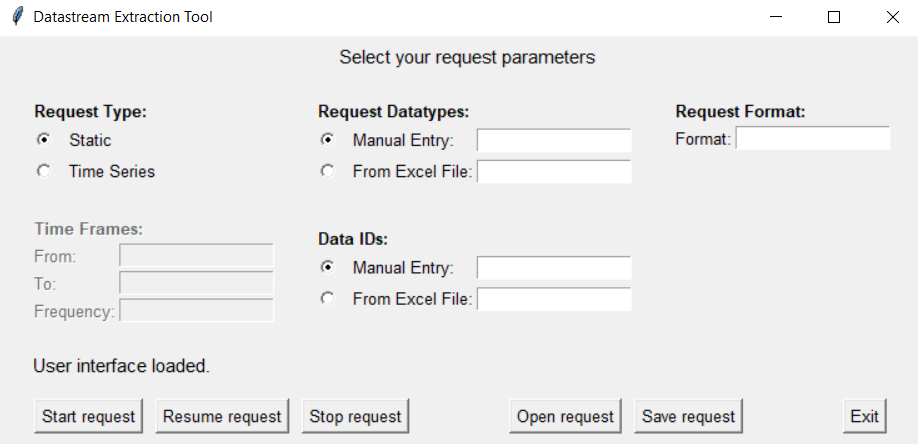
\includegraphics[width=1.1\linewidth]{figures/gui.png}
	\caption{Graphical User Interface of the Datastream Extraction Tool}
	\label{fig:gui-2}
\end{figure}

In the \textbf{Request Type} section you can select your request to encompass either static or time-series data for the stocks or bonds that you want to download. \\

If you select the option \textit{Time Series}, the \textbf{Time Frames} section will become enabled. There, you can enter the start and the end date of the period for which you want to download data. The dates have to be entered in the format "dd/mm/yy" (e.g. 01/01/99 for the 1st of January 1999, or 30/06/20 for the 30th of June 2020). The program assigns year numbers from 51 to 99 automatically to the years 1951 - 1999, and year numbers from 00 to 50 to the years 2000 - 2050. 
In the \textit{Frequency} text field, you can type in the frequency of the time points that you want to get. Here, the values "Daily", "Weekly", "Monthly", "Quarterly", and "Yearly" are allowed. \\

Within the \textbf{Request Datatypes} section, you can enter the codes of the parameter types that you want to get for your stocks or bonds. These could be e.g. "C" for coupon, or "ISIN". You can enter the values either manually, or by choosing the excel file from which you want to get the datatypes. If you choose to enter the datatype codes manually, please do so in a comma-separated manner (e.g. "C,ISIN,AIS,BSTAT"). If you choose to enter the codes via excel file, you have to create an excel file with all the datatype codes listed in column A, one below the other (see Fig. \ref{fig:file-datatypes}). Then, within the app, browse for the created file and select it.

\begin{figure}[h]
	\centering
	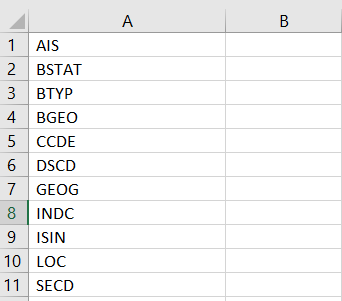
\includegraphics[width=0.4\linewidth,height=0.35\linewidth]{figures/enter-datatypes.png}
	\caption{A sample file with datatypes}
	\label{fig:file-datatypes}
\end{figure}

In the \textbf{Data IDs} section, you have to enter the datastream codes of the financial instruments - i.e. stocks or bonds - that you are interested in. Just like for datatypes, this can be done either manually, or by giving the excel file name, in which you have previously stored the IDs. When entering them manually, separate the IDs by commas again. When entering them via file, store them in the A column of your excel document, like before, and select the created file in the app by clicking on the "Browse" button. \\

In the \textbf{Request Format} section you can (optionally) enter the format in which you want your data to appear. You can give the format by concatenating the letters of the different format options available in Datastream. For example, "CRM\$" would mean to include column headers (C), row headers (R), instrument code (M), and currency (\$). \\

Finally, in the \textbf{Save Results To} section of the interface you can enter the folder location to which you want your request results to be saved. For this, either enter a valid folder path by hand, or select it by clicking on the button to browse for a suiting folder. \\

Below the parameter sections, there is a \textbf{status bar} that shows you the current status of your request. This can be especially useful for longer requests. Please keep in mind that the status bar can have a delay of up to 2 minutes, depending on the current request phase. For real-time request updates, please refer to Logs in the Folder Structure section of this guide. \\

Additionally, at the bottom of the gui, there are several control buttons. The "\textbf{Start Request}" button first checks the format of the fields you entered, and subsequently launches the request. The current status of the request will be shown in the status bar. \\


The "\textbf{Stop Request}" button shuts down the request if there is one currently running. In its essence, it kills the running Excel instance to stop the data download. Depending on the phase of the request, it might take up to 2 minutes until the request has been stopped. Please abstain from using the gui during this time. \\


The "\textbf{Resume Request}" button is there to resume a request that was previously started and then stopped. This action ignores any entered parameter fields, as it simply resumes the last request, with the settings it has internally saved. Requests that were resumed automatically continue to download data, starting from the last data chunk that has previously been downloaded. Use the "Resume Request" button if your download crushed or if you stopped it manually. \\


The "\textbf{Open Request}" and "\textbf{Save Request}" buttons are there to either save current parameters into a file, or to conveniently load request parameters from a file. Use this for recurring requests to avoid entering them by hand each time. \\


Finally, the "\textbf{Exit}" button first stops the request if there is one running, and then closes the application. If you want to close the application without stopping the request, close the window as usually with the cross at the top right of the window. Note that in this case Excel might proceed running in the background!

\subsection{Application Folders}
The application is shipped with several folders that it requires to run. These are: 

\begin{itemize}
	\item Data
	\item DataTypes
	\item IDs
	\item Logs
	\item PythonPackages
	\item Requests
	\item Settings
\end{itemize}

In \textbf{Data}, the downloaded data from the users' requests is getting stored. It is stored in the form of Excel files. The number of files varies depending on the request size. The file size is centered around 40 MB each, but can also vary, depending on the particular request and the available data. You can use the files with downloaded data for whichever purpose you want. It is advisable though to avoid further manipulating these files in-place, and rather to copy them elsewhere for further processing. \\

In the \textbf{DataTypes} folder, you can put Excel files with the datatypes of financial instruments that you want to download. These have to be stored in column A, one datatype per row. The application is shipped with several examples. \\

In \textbf{IDs}, you can put Excel files containing Datastream identifiers of financial instruments, for which you would like to download data. Just like for datatypes, you have to store these in the A column of the respective Excel file, one ID per row. Refer to section IDs Preparation for hints on how to do it conveniently. \\

In the folder \textbf{Logs}, you will find two files, which are generated when the program is running. The first one is called \textit{log\_python.txt}. It contains real-time information on the progress of the data download. Use the file to either check the current download status, or to track occurring errors, should the application misbehave. The second file is called \textit{log\_request\_table.txt}. It contains real-time information on the progress of the data download on the Excel side of the program (i.e in the request table). You can similarly use it either for progress updates, or for troubleshooting. \\

The folder \textbf{PythonPackages} is of technical nature. It contains python packages that are needed for the application to run. Please, do not touch this folder, unless you know what you are doing. \\

In the folder \textbf{Requests}, you can store parameters of previous requests, in order to reuse these later. The requests are stored .txt files. The file names you can choose yourself at creation. \\

The folder \textbf{Setting}s contains one single file called \textit{settings.txt}. This file is used for multiple purposes, including: 

\begin{itemize}
	\item communication between the python and the excel part of the application
	\item download progress monitoring
	\item error monitoring
	\item status updates in the gui
	\item the "resume request" functionality
\end{itemize}
The settings and communication data within the file is stored in the key-value-format. In most cases, you should \textbf{not} open or modify the file. For exceptions, refer to the Troubleshooting section. 

\subsection{Troubleshooting}

\subsubsection{3.3.1 Thomson Reuters Eikon add-in does not show in the list of active Excel add-ins}
\textbf{Problem Description: }  \\
Thomson Reuters Eikon add-in does not show in the list of active Excel add-ins. \\ \\
\textbf{Solution Proposal:} \\
In the \textit{RequestTable.xlsm} document, navigate to File $ => $ Options $ => $ Add-ins. If the add-in is listed under "Deactivated Application Add-ins" in the Add-ins tab of Options, then at the bottom select \textit{Manage: Deactivated elements} and click on "Go". In the appearing window, if the Thomson Reuters add-in is listed, check it and click on "Activate". \\
If the Reuters add-in is listed under "Inactive Application Add-ins" instead, then at the bottom select \textit{Manage: COM Add-ins} and click "Go". In the appearing window, if \textit{Thomson Reuters Eikon - Microsoft Office} is not checked, check it. If the Reuters add-in is not in the list, click on "Add" and navigate to the add-in location. In many cases, it is stored under 
\url{C:\\Users\\[current_user]\\AppData\\Local\\ThomsonReuters\\Eikon\\EikonOfficeShim.dll}. 
Select it and add it to the list. If not, find out where the file \textit{EikonOfficeShim.dll} is stored on your computer and add it to the list of add-ins. 

\subsubsection{3.3.2 Sign-In Problems with Thomson Reuters Eikon Add-in}
\textbf{Problem Description: }  \\
The Excel add-in of Thomson Reuters Eikon \& Datastream sometimes logs-out for unclear reasons, or because a different user logged-in with the same account data. In most cases, this results in an Excel message during download, which states that the user is not signed-in to Thomson Reuters. \\ \\
\textbf{Solution Proposal:} \\
Sign-in to Thomson Reuters manually in Excel. Then restart or resume the download. If this does not solve the issue, try restarting Windows. 

\subsubsection{3.3.3 Download Problems}
\textbf{Problem Description: }  \\
One of the following hanging problems applies: 
\begin{itemize}
	\item The download seems to hang, but the app does not recognize it. 
	\item The app recognized the hanging, but cannot shut down the download. 
	\item The app shut down the download due to hanging, but Excel keeps running. 
	\item You stopped the request manually, but it seems to still be running. 
	Neither the app, nor Excel respond, or the entire computer seems to hang. 
\end{itemize} 
\textbf{Solution Proposal:} \\
Open Task Manager. Kill the Excel task first, then the extraction tool. The extraction tool will be shown as "Python" in the task list. Then restart the extraction tool and resume the download. 

\section{Technical Aspects} \label{appendix:technical-aspects}
In this section, a technical description of the application architecture will be provided. For an illustration of the entire architecture, see Fig. \ref{fig:ds-extraction-tool-arch}. 
\begin{figure}[h]
	\centering
	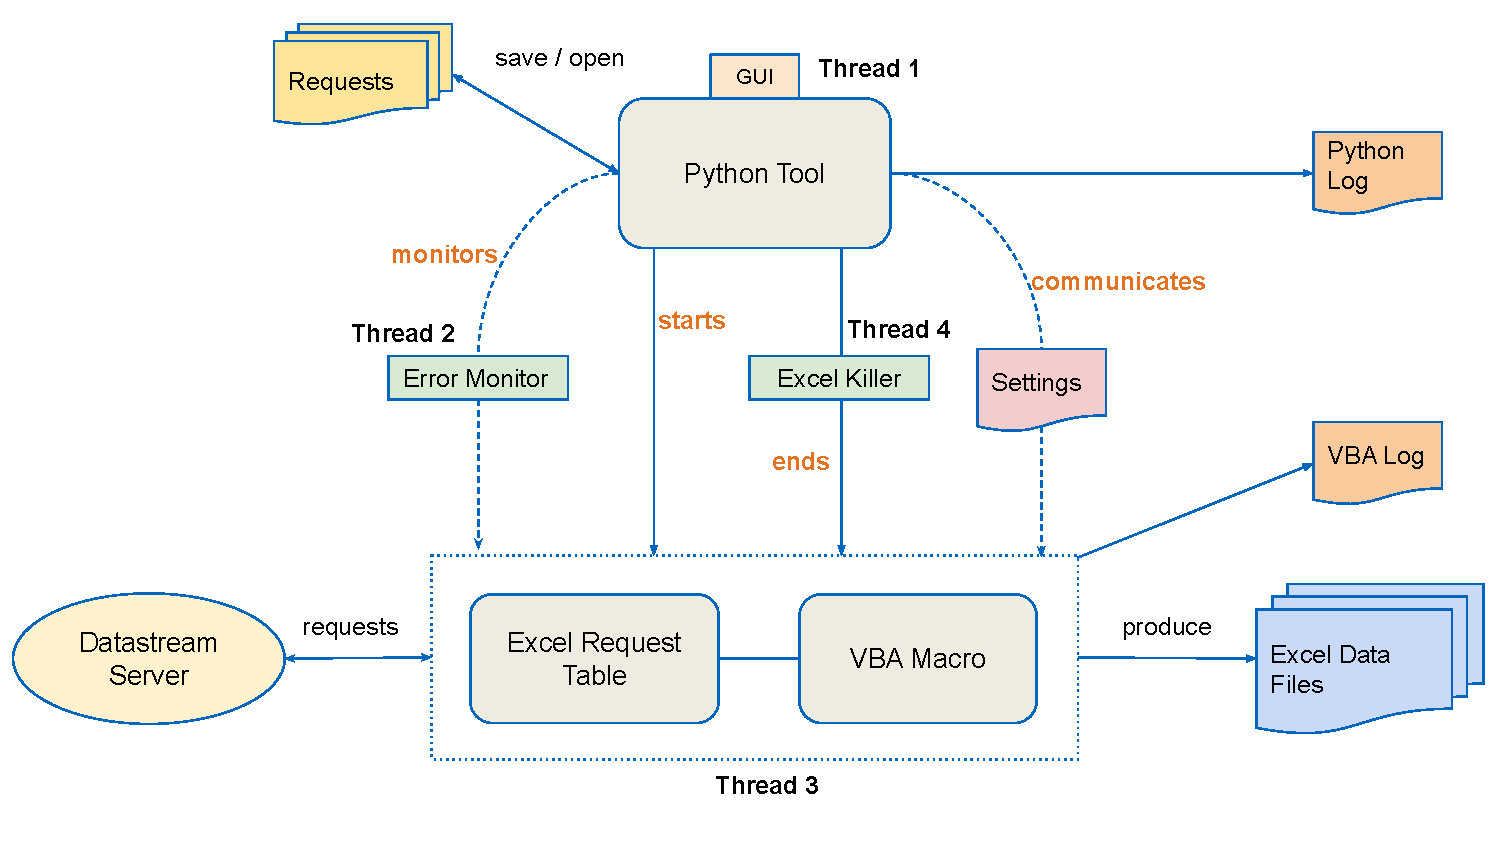
\includegraphics[width=1.1\linewidth]{figures/ds-extraction-tool-architecture}
	\caption{Datastream Extraction Tool Architecture}
	\label{fig:ds-extraction-tool-arch}
\end{figure}

\subsection{Excel / VBA Part}
The Visual Basic for Applications part of the data extraction tool consists of four modules, each serving its own purpose: 
\begin{itemize}
	\item modDeclares
	\item modVariables
	\item modUtils
	\item modTS
\end{itemize}
Within \textit{modDeclares}, operating system level constants and functions are defined. The declaration of such functions with \textit{Declare} and of constants with \textit{Const} equals an import of this functionality to the project. If you are not familiar with the reasoning behind the usage of \textit{PtrSafe} and \textit{LongPtr} keywords, you can read it up here: .  \\ %TODO
%https://docs.microsoft.com/en-us/office/vba/language/reference/user-interface-help/ptrsafe-keyword
%https://docs.microsoft.com/en-us/office/vba/language/reference/user-interface-help/longptr-data-type

The module \textit{modVariables} simply contains all the global variables used within the project, split by their usage area as described in the annotations. \\

In \textit{modUtils}, a large amount of helper functions are defined. About half of them are self-written, the others come from solutions available online. While I cannot guarantee for all of them to always work correctly, it is unlikely for them to contain bugs, since I extensively tested most of them in different contexts. 
The most important functions are the ones I wrote to wrap the communication with the \textit{settings.txt} file (InitDict, GetFromDict, UpdateDict, PutKV, and GetKV), and those responsible for the Datastream Add-In connection (Connect\_COM\_AddIn, InstallCOMAddIn, iAddInStatus, CheckPluginConnection). Make sure to familiarize yourself with them if you are going to make changes or extensions to the tool. \\

The module \textit{modTS} is the main module of the tool, in which most of the action happens. It is well-modularized by itself and contains the following functions: 
\begin{itemize}
	\item getTSData
	\item start
	\item init
	\item setDefaultSettings
	\item getIDs
	\item getDatatypes
	\item doCalculations
	\item fillTableIDs
	\item fillTableFields
	\item request
\end{itemize}
The order of execution when the tool is started directly corresponds with the position of the functions in the code (like above). \textit{getTSData} is the only function declared as \textit{public} in the module, and is the entry point to the program. This function gets called from the Python part of the tool whenever a request has been started by the user. It calls the function \textit{start}, which sets default constants, checks the Datastream add-in connection, unpacks user-provided settings from the \textit{settings.txt} file, and calls the \textit{init} function if this is the first time this request is executed. The \textit{first\_time} is set in the \textit{settings.txt} file originally, and is received from there via the key-value dictionary wrapper. If this is the first time one and the same request is being started, the function \textit{init} initializes global variables with values from the settings dictionary. Additionally, the function initializes a number of other functions which fill the request table with contents needed to execute the user request. \\

At first, the current request table sheet is cleared from previous contents (\textit{ClearCurrentSheet}). Then, data identifiers are loaded from the user-provided file with IDs (\textit{getIDs}). After that, the same is being done with datatypes (\textit{getDatatypes}). Having received all the required input data, some calculations are being carried out (\textit{doCalculations}), which are there to estimate the optimal number of identifiers for a single request to Datastream. This is necessary, because Datastream has a maximum request size, both by number of submitted IDs and by the amount of data downloaded. Make sure you fully understand the calculations before making changes to this function. It is the likely the most complex one in the entire program. \\

As the next step, the request table gets filled with contents. For this purpose, first the function \textit{fillTableIDs}, and then \textit{fillTableFields} is executed. \\

After all these steps have been carried out, the actual download of the data starts. It is initiated in the main function \textit{getTSData} for each of the parts that need to be downloaded. A single request is being handled by the function \textit{request}. This is the only place in the code, where the call to the actual Datastream API happens via the provided interface function \textit{btnProcessTable\_Click}. The function itself can be found in the \textit{basEvents} module, which is always available in a Datastream request table by default. \\

In terms of additional functionality, the tool provides logging throughout the code to enable troubleshooting when needed. The logs are stored in the \textit{Logs} folder of the tool. 

\subsection{Python Part} 
In order to fully understand the architecture of the Python side of the application, take a look at Fig. \ref{fig:ds-extraction-tool-arch} again. The main point of entry into the user-side application is the user interface (gui). It runs on the main thread of the program, and is maintained by the module called \textit{ds\_extraction\_tool}. The user interface has been created with the package \textit{Tkinter}. %TODO ref Tkinter package
It provides a way to relatively fast create user interfaces, even though they are not very flexible in terms of appearance. Most of the \textit{ds\_extraction\_tool} module deals with gui elements and user interaction with them. \\

The most interesting functions are start\_\textit{request}, \textit{resume\_request} and \textit{stop\_request}. start\_\textit{request} and \textit{resume\_request} both put user-defined request settings, which were previously entered by the user in the user interface, into the \textit{settings.txt} file, which in its turn is used to communicate with the VBA part of the program. The settings file on the Python file is wrapped into a key-value dictionary, similarly to the way it is done in VBA. The dictionary implementation is self-made and can be found in the module \textit{kv\_file\_manager}.  \\

After filling the settings file with user contents, a new thread (Thread 2) gets started, in which the module \textit{excel\_controller} runs. The module is responsible for starting up Excel, and for submitting the actual download request to VBA. A new thread is needed in order to keep the gui responsive throughout the download. Additionally, the module performs error monitoring and progress control at runtime. This is the most complex module on the Python side of the program. Take some time to familiarize yourself with it. The module receives the call from \textit{ds\_extraction\_tool} which lands in the \textit{start} function. The \textit{start} function, in its turn, calls the \textit{run} function. The \textit{run} function creates a new thread (Thread 3), in which Excel is started, the request table opened, and the VBA macro \textit{getTSData} launched. In order to submit all this to Thread 3, this functionality needs to be wrapped in a non-class function called \textit{run\_rt}, also available in the module. \\

After the VBA macro and thus the download have been launched, the module \textit{excel\_controller} keeps monitoring the execution by regularly checking the contents of the \textit{settings.txt} file. This is done by the two boolean functions \textit{finished\_request} and \textit{download\_hangs}. If the module notices that the download has finished (by comparing currently downloaded data part with total number of parts in the settings file), it stops the execution and issues a message to the user that the download has completed. If it notices that the download is likely hanging (by reaching a counter timeout on the same data part being downloaded for a long time), Excel, and thus the running macro, gets killed so that the hanging download can be stopped. This is handled by the module \textit{excel\_killer}. The process responsible for stopping Excel also runs on a separate thread (Thread 4), in order to prevent interference with the \textit{excel\_controller} module and the gui. After that, Excel gets restarted, the request table reopened, and the download resumed at the same download stage where it was interrupted. \\

Additionally, the Python side of the application also writes a log, which can be found in the \textit{Logs} folder of the application, and delivers download status updates to the gui module to notify the user of what is currently happening. The latter is done over the object called \textit{obj\_update}, which is reached over to the \textit{excel\_controller} module by the gui when the user request is being forwarded to Thread 2. \\

The module \textit{variables} stores all the global variables utilized on the Python side. The module \textit{registry\_killer} is there to kill a registry entry Excel keeps settings when the Datastream add-in misbehaves. If the entry is not deleted at each program start, it might be that the Datastream add-in is blacklisted by Excel, and thus cannot start. The functionality is essential for the tool to work reliable. Finally, the module \textit{log\_file\_manager} is responsible for writing the log file. 

%\input{chapters/AppendixDoFiles}

\chapter{Lead-Lag Regression Results} \label{appendix-regression}
\captionsetup{margin=10pt,font=large,labelfont=bf,textfont={bf}}

\section{By Geography}

\begin{figure}[H]
	\centering
	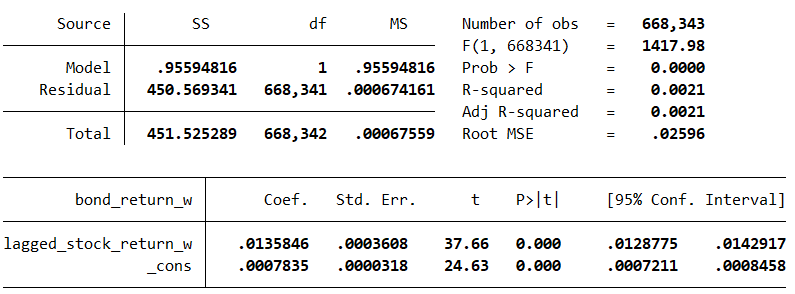
\includegraphics[width=1.0\linewidth]{figures/regression-results/regression-world-bonds-as-dependent.PNG}
	\caption{Regression result: World; bonds as dependent, lagged stocks as independent variable. }
	\label{fig:regression-world-bonds-as-dependent}
\end{figure}

\begin{figure}[H]
	\centering
	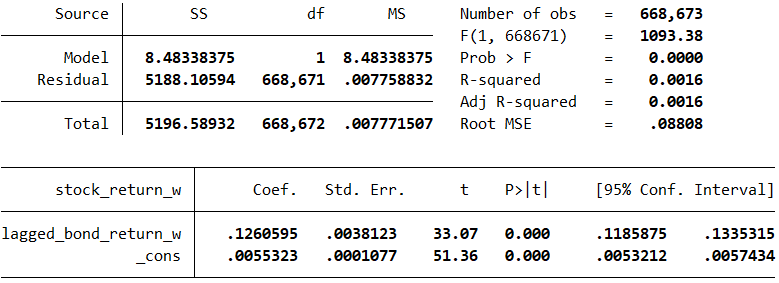
\includegraphics[width=1.0\linewidth]{figures/regression-results/regression-world-stocks-as-dependent.PNG}
	\caption{Regression result: World; stocks as dependent, lagged bonds as independent variable. }
	\label{fig:regression-world-stocks-as-dependent}
\end{figure}

\begin{figure}[H]
	\centering
	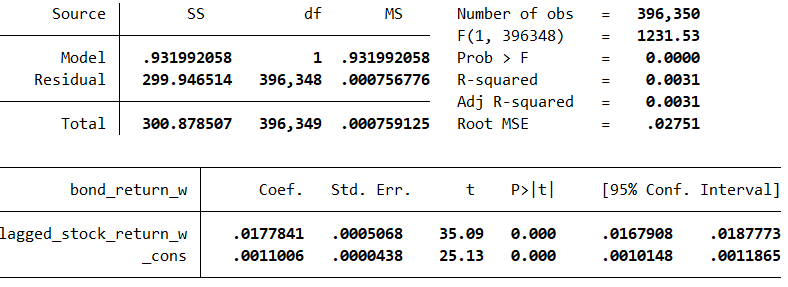
\includegraphics[width=1.0\linewidth]{figures/regression-results/regression-na-bonds-as-dependent.PNG}
	\caption{Regression result: U.S. \& Canada; bonds as dependent, lagged stocks as independent variable. }
	\label{fig:regression-na-bonds-as-dependent}
\end{figure}

\begin{figure}[H]
	\centering
	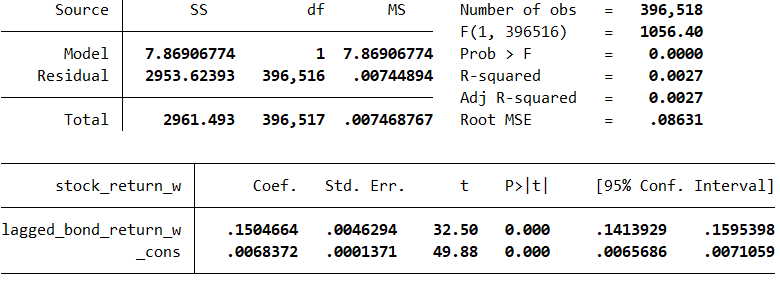
\includegraphics[width=1.0\linewidth]{figures/regression-results/regression-na-stocks-as-dependent.PNG}
	\caption{Regression result: U.S. \& Canada; stocks as dependent, lagged bonds as independent variable. }
	\label{fig:regression-na-stocks-as-dependent}
\end{figure}

\begin{figure}[H]
	\centering
	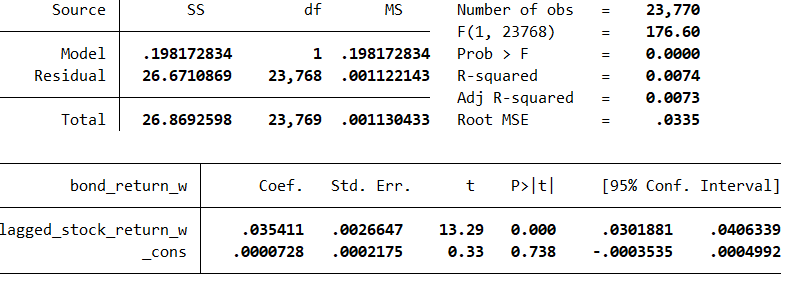
\includegraphics[width=1.0\linewidth]{figures/regression-results/regression-sa-bonds-as-dependent.PNG}
	\caption{Regression result: South America; bonds as dependent, lagged stocks as independent variable. }
	\label{fig:regression-sa-bonds-as-dependent}
\end{figure}

\begin{figure}[H]
	\centering
	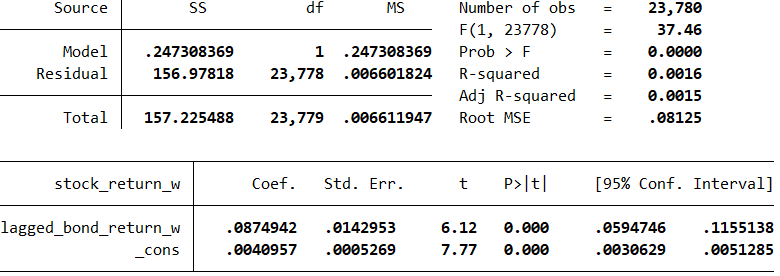
\includegraphics[width=1.0\linewidth]{figures/regression-results/regression-sa-stocks-as-dependent.PNG}
	\caption{Regression result: South America; stocks as dependent, lagged bonds as independent variable. }
	\label{fig:regression-sa-stocks-as-dependent}
\end{figure}

\begin{figure}[H]
	\centering
	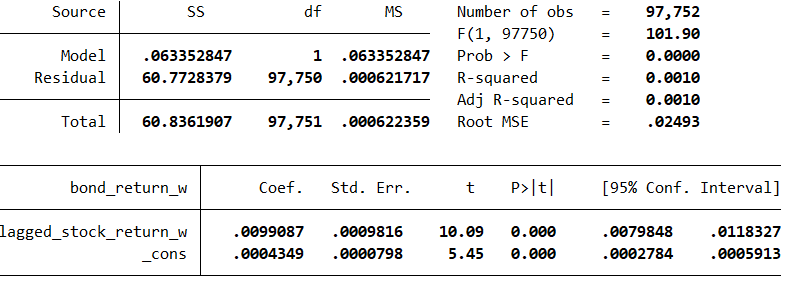
\includegraphics[width=1.0\linewidth]{figures/regression-results/regression-euw-bonds-as-dependent.PNG}
	\caption{Regression result: Western Europe; bonds as dependent, lagged stocks as independent variable. }
	\label{fig:regression-euw-bonds-as-dependent}
\end{figure}

\begin{figure}[H]
	\centering
	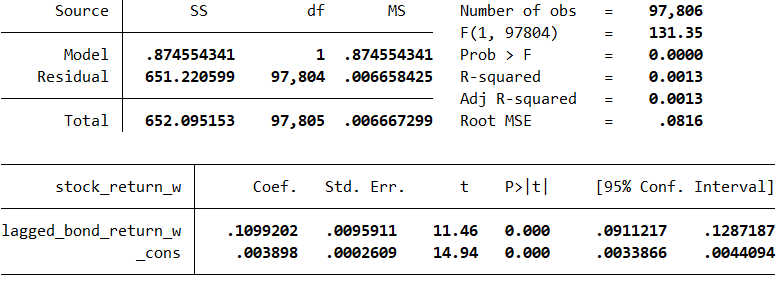
\includegraphics[width=1.0\linewidth]{figures/regression-results/regression-euw-stocks-as-dependent.PNG}
	\caption{Regression result: Western Europe; stocks as dependent, lagged bonds as independent variable. }
	\label{fig:regression-euw-stocks-as-dependent}
\end{figure}

\begin{figure}[H]
	\centering
	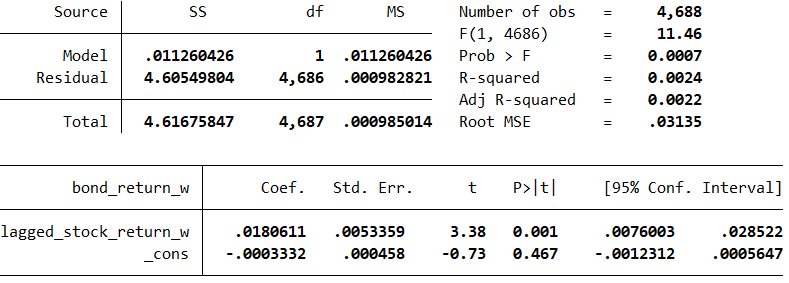
\includegraphics[width=1.0\linewidth]{figures/regression-results/regression-eue-bonds-as-dependent.PNG}
	\caption{Regression result: Eastern Europe; bonds as dependent, lagged stocks as independent variable. }
	\label{fig:regression-eue-bonds-as-dependent}
\end{figure}

\begin{figure}[H]
	\centering
	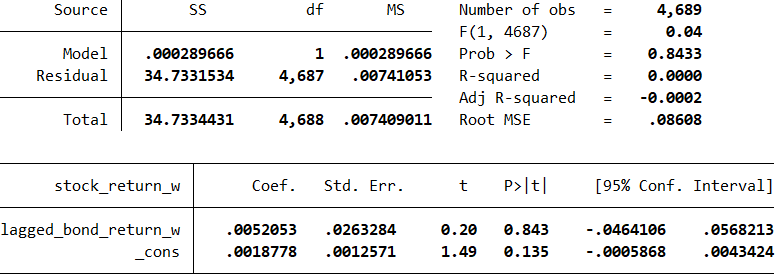
\includegraphics[width=1.0\linewidth]{figures/regression-results/regression-eue-stocks-as-dependent.PNG}
	\caption{Regression result: Eastern Europe; stocks as dependent, lagged bonds as independent variable. }
	\label{fig:regression-eue-stocks-as-dependent}
\end{figure}

\begin{figure}[H]
	\centering
	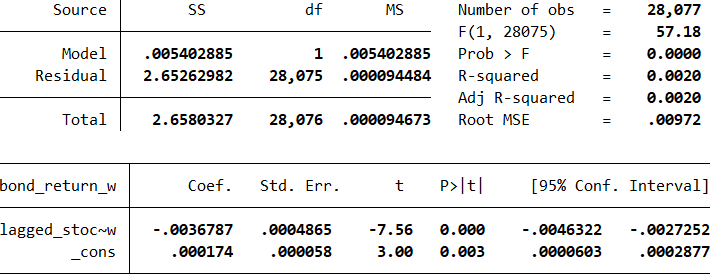
\includegraphics[width=1.0\linewidth]{figures/regression-results/regression-china-bonds-as-dependent.PNG}
	\caption{Regression result: China; bonds as dependent, lagged stocks as independent variable. }
	\label{fig:regression-china-bonds-as-dependent}
\end{figure}

\begin{figure}[H]
	\centering
	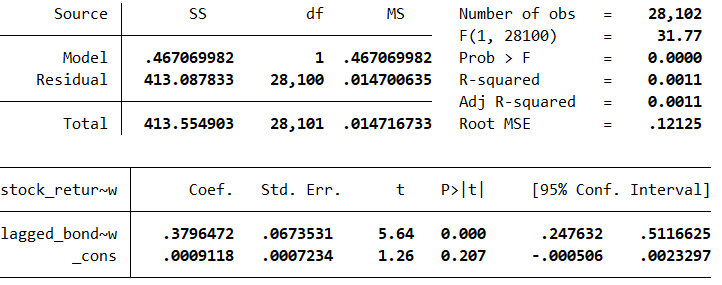
\includegraphics[width=1.0\linewidth]{figures/regression-results/regression-china-stocks-as-dependent.PNG}
	\caption{Regression result: China; stocks as dependent, lagged bonds as independent variable. }
	\label{fig:regression-china-stocks-as-dependent}
\end{figure}

\section{By Credit Rating}
For brevity purposes, the lead-lag regression results for bond groups split by credit rating are provided separately, and can be found in the project folder in the \textbf{Statistics} part.

\section{By Aggregated Credit Rating}
\begin{figure}[H]
	\centering
	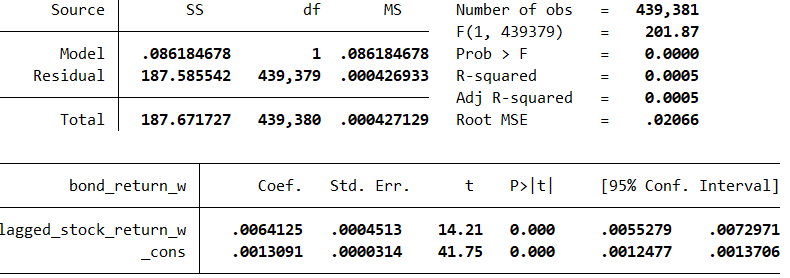
\includegraphics[width=1.0\linewidth]{figures/regression-results/regression-investment-grade-bonds-as-dependent.PNG}
	\caption{Regression result: Investment Grade Bonds; bonds as dependent, lagged stocks as independent variable. }
	\label{fig:regression-investment-grade-bonds-as-dependent}
\end{figure}

\begin{figure}[H]
	\centering
	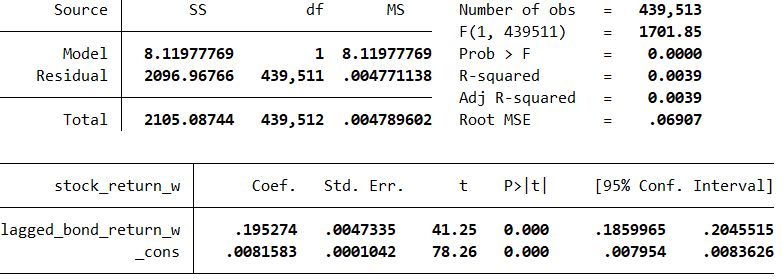
\includegraphics[width=1.0\linewidth]{figures/regression-results/regression-investment-grade-stocks-as-dependent.PNG}
	\caption{Regression result: Investment Grade Bonds; stocks as dependent, lagged bonds as independent variable. }
	\label{fig:regression-investment-grade-stocks-as-dependent}
\end{figure}

\begin{figure}[H]
	\centering
	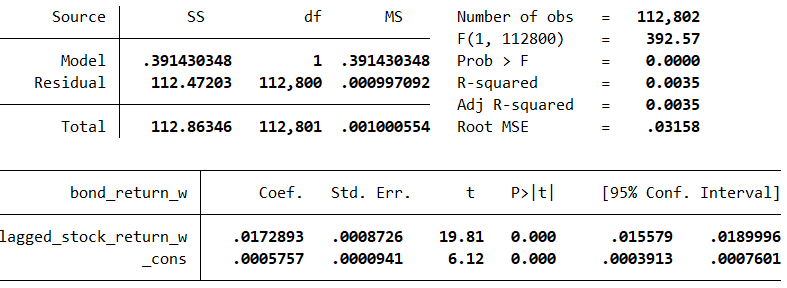
\includegraphics[width=1.0\linewidth]{figures/regression-results/regression-non-investment-grade-bonds-as-dependent.PNG}
	\caption{Regression result: Non-Investment Grade Bonds; bonds as dependent, lagged stocks as independent variable. }
	\label{fig:regression-non-investment-grade-bonds-as-dependent}
\end{figure}

\begin{figure}[H]
	\centering
	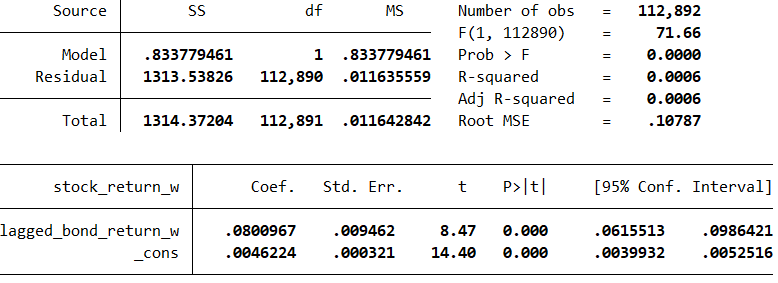
\includegraphics[width=1.0\linewidth]{figures/regression-results/regression-non-investment-grade-stocks-as-dependent.PNG}
	\caption{Regression result: Non-Investment Grade Bonds; stocks as dependent, lagged bonds as independent variable. }
	\label{fig:regression-non-investment-grade-stocks-as-dependent}
\end{figure}

\section{High Yield}

\begin{figure}[H]
	\centering
	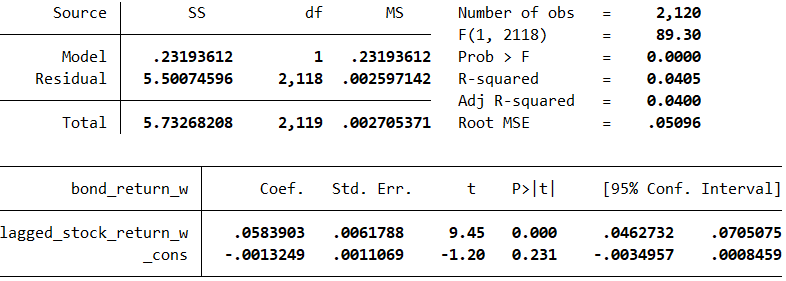
\includegraphics[width=1.0\linewidth]{figures/regression-results/regression-high-yield-ccc-d-moodies-bonds-as-dependent.PNG}
	\caption{Regression result: High Yield Bonds by Moody's (Ca \& C); bonds as dependent, lagged stocks as independent variable. }
	\label{fig:regression-high-yield-moodys-bonds-as-dependent}
\end{figure}

\begin{figure}[H]
	\centering
	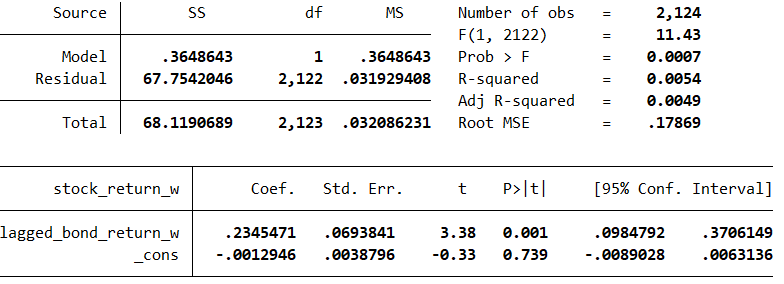
\includegraphics[width=1.0\linewidth]{figures/regression-results/regression-high-yield-ccc-d-moodies-stocks-as-dependent.PNG}
	\caption{Regression result: High Yield Bonds by Moody's (Ca \& C); stocks as dependent, lagged bonds as independent variable. }
	\label{fig:regression-high-yield-moodys-stocks-as-dependent}
\end{figure}

\begin{figure}[H]
	\centering
	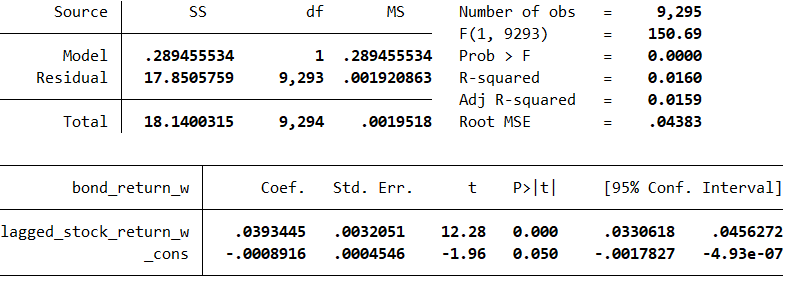
\includegraphics[width=1.0\linewidth]{figures/regression-results/regression-high-yield-sandp-bonds-as-dependent.PNG}
	\caption{Regression result: High Yield Bonds by S\&P (CCC); bonds as dependent, lagged stocks as independent variable. }
	\label{fig:regression-high-yield-sandp-bonds-as-dependent}
\end{figure}

\begin{figure}[H]
	\centering
	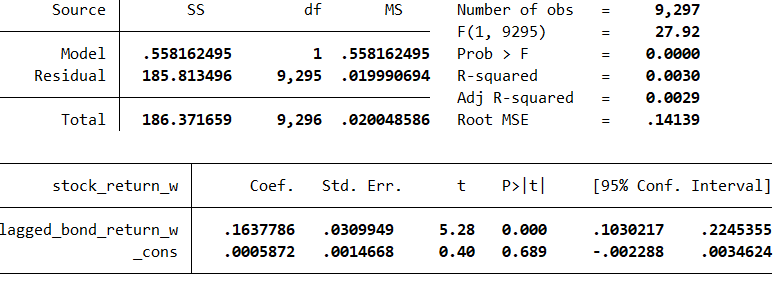
\includegraphics[width=1.0\linewidth]{figures/regression-results/regression-high-yield-sandp-stocks-as-dependent.PNG}
	\caption{Regression result: High Yield Bonds by S\&P (CCC); stocks as dependent, lagged bonds as independent variable. }
	\label{fig:regression-high-yield-sandp-stocks-as-dependent}
\end{figure}






